\subsection{Адаптация CbmRoot для работы с GDML}\label{sec:secFairModule}

\todo -----------------------------------------------------------------

На данный момент в FairRoot в классе FairModule присутствуют методы
ConstructGDMLGeometry - вызывает parser.GDMLReadFile, ReAssignMediaId, ExpandNodeForGDML
ConstructASCIIGeometry
ConstructRootGeometry - с реализацией
ConstructGeometry - пустой, нужен для реализации в дочерних классах
ConstructOpGeometry - пустой, нужен для реализации в дочерних классах
ModifyGeometry - ? 

ExpandNode
ExpandNodeForGDML

ReAssignMediaId
AssignMediumAtImport

Сделан отлов ситуации, если GDML не был включён при установке.

В CbmRoot также имеется класс CbmModule, унаследованный от FairModule с методами ConstructGDMLGeometry и ExpandNodeForGDML, по-видимому, давно не обновлявшиеся.

CbmRich унаследован от FairDetector

\todo -----------------------------------------------------------------

% \todo
\textbf{Я просто перенёс текст из диплома с небольшими изменениями. Боюсь, к настоящему моменту, ситуация заметно изменилась...}

Целевым пакетом для большинста MC-моделей, разработанных с помощью ``CATIA-GDML geometry builder'', в частности CBM RICH, является пакет CbmRoot, в котором выполняется моделирование, реконструкция, приём и анализ данных эксперимента CBM. CbmRoot является фреймворком, написанным на основе FairRoot, который в свою очередь написан на основе ROOT.

Любой элемент экспериментальной установки в системе FairROOT описывается классом, наследованным от базового класса \classname{FairModule}. Для импорта геометрической информации из внешнего файла предусмотрен метод \methodname{ConstructGeometry} класса \classname{FairModule}. Данный метод не выполняет непосредственно чтение информации, а лишь определяет тип файла и выбирает какой метод необходимо вызвать.

Поддерживаются различные форматы входных файлов, поэтому существуют отдельные методы, отвечающие за соответствующие форматы:

\begin{itemize}
\itemsep0pt
\item \methodname{ConstructROOTGeometry};
\item \methodname{ConstructASCIIGeometry};
\item \methodname{ConstructGEOGeometry}.
\end{itemize}

Данные методы могут быть имплементированы на различных уровнях --- как в базовом классе \classname{FairModule}, так и конечном, описывающем конкретный элемент, или в любом промежуточном классе, если таковые имеются.

В данной секции в качестве конкретного элемента экспериментальной установки будем рассматривать детектор RICH эксперимента CBM. Соответствующий класс имеет название \classname{CbmRich}. Всё описание с незначительными дополнениями распространяется на любой активный либо пассивный элемент установки (далее детектор).

На \figref{fig:classesBefore} представлена диаграмма, отражающая иерархию классов и методов, касающихся импорта геометрии до внесения изменений.

\begin{figure}[H]
\centering
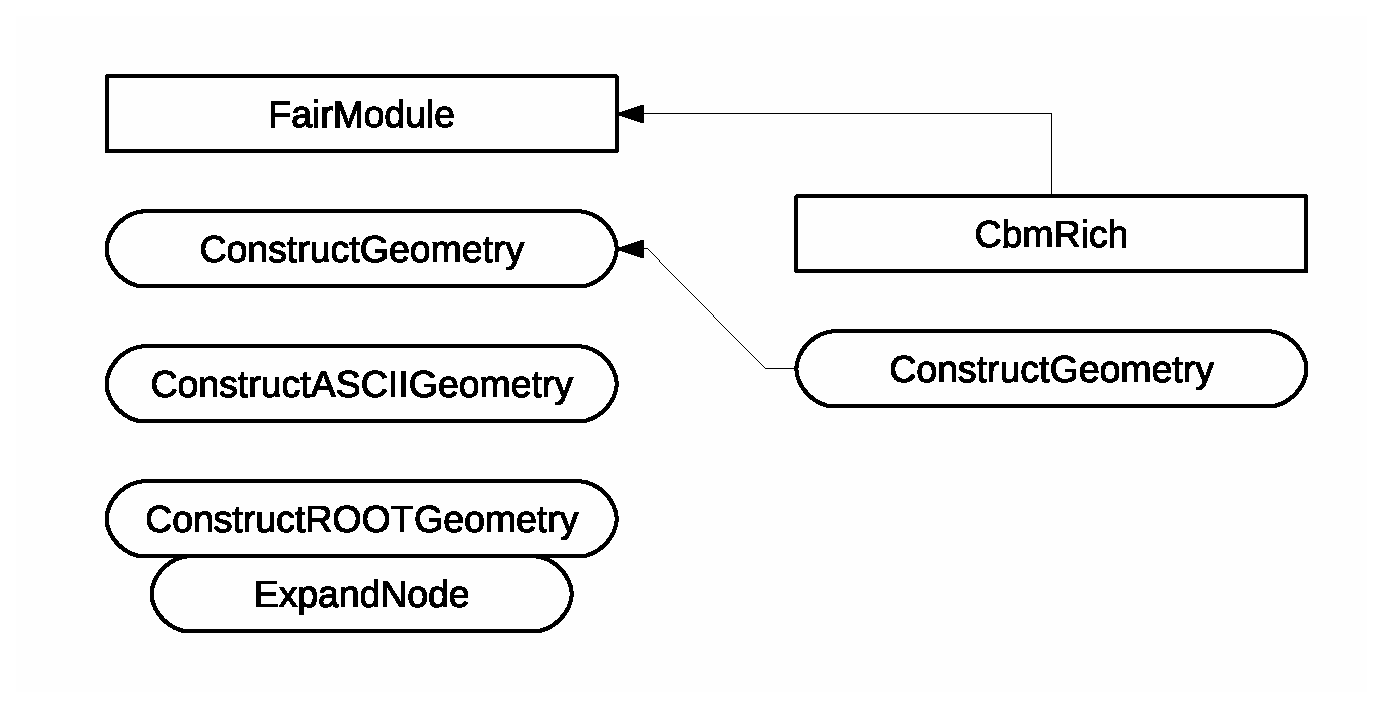
\includegraphics[width=0.7\textwidth]{pictures/FairModule_classes_before.eps}
\caption{Диаграмма классов CbmROOT до модификации.}
\label{fig:classesBefore}
\end{figure}

Если метод объявлен в материнском классе, то он может быть определён (т.е. собственно его код написан) как в дочернем классе, так и в материнском.

Метод \methodname{ConstructGeometry} объявлен в \classname{FairModule}, но определён всегда в классе детектора. Именно этот класс определяет, какой метод вызывать в зависимости от формата входного файла. Метод \methodname{ConstructASCIIGeometry} объявлен в \classname{FairModule}, но не реализован в дочернем классе \classname{CbmRich}. Это означает, что для детектора RICH не предусмотрен импорт из текстового файла, но существует какой-то другой элемент установки, который имеет описание импорта из формата ASCII.

Первоначально был введён метод \methodname{ConstructGDMLGeometry} на уровне класса \classname{FairModule}. Таким образом для того чтобы обеспечить вызов этого метода из класса детектора, достаточно было лишь добавить условие в методе \methodname{ConstructGeometry} в классе детектора. Автоматически вызывался бы метод из FairROOT. Такой подход был реализован и успешно проверен на локальной установке CbmRoot. Однако когда введённые изменения были внесены в промежуточный (trunk) вариант пакета в GSI было обнаружено, что возникают сложности, вызывающие некорректную работу других модулей пакета.

Для работы импорта из GDML файла необходима определённая динамическая библиотека. Эта библиотека не скомпилирована по умолчанию. Если изменить исходный код FairROOT необходимо скомпилировать упомянутую библиотеку и поместить её в соответствующую папку FairROOT. По той причине, что имеется множество наследованных от FairROOT пакетов и ни один из них не скомпилирован с поддержкой GDML, изменения в исходном коде потребуют перекомпиляции всех дочерних программ, что представляет собой трудоёмкую процедуру, требующую прав администратора и значит недопустимую на данном этапе.

Было принято решение временно перенести исходный код импорта из GDML в новый промежуточный класс \classname{CbmModule}. Затем в определённый момент, спустя годы, описываемый функционал был включён в FairRoot, что позволило использовать GDML как формат импортируемой геометрии всем унаследованным от FairRoot пакетам --- R3BRoot, PandaRoot, и т.д.

%После длительного обсуждения с разработчиками FairROOT и CbmROOT было принято решение перенести исходный код импорта из GDML в новый класс \classname{CbmModule}, что позволило внести изменения только в CbmROOT и избежать неполадок.
%Описанная процедура может быть применена к любому пакету, наследованному от FairROOT, однако на данном этапе изменения включены только в CbmROOT. Рассматривается перспектива внедрения GDML и в пакет R3BROOT.

\begin{figure}[H]
\centering
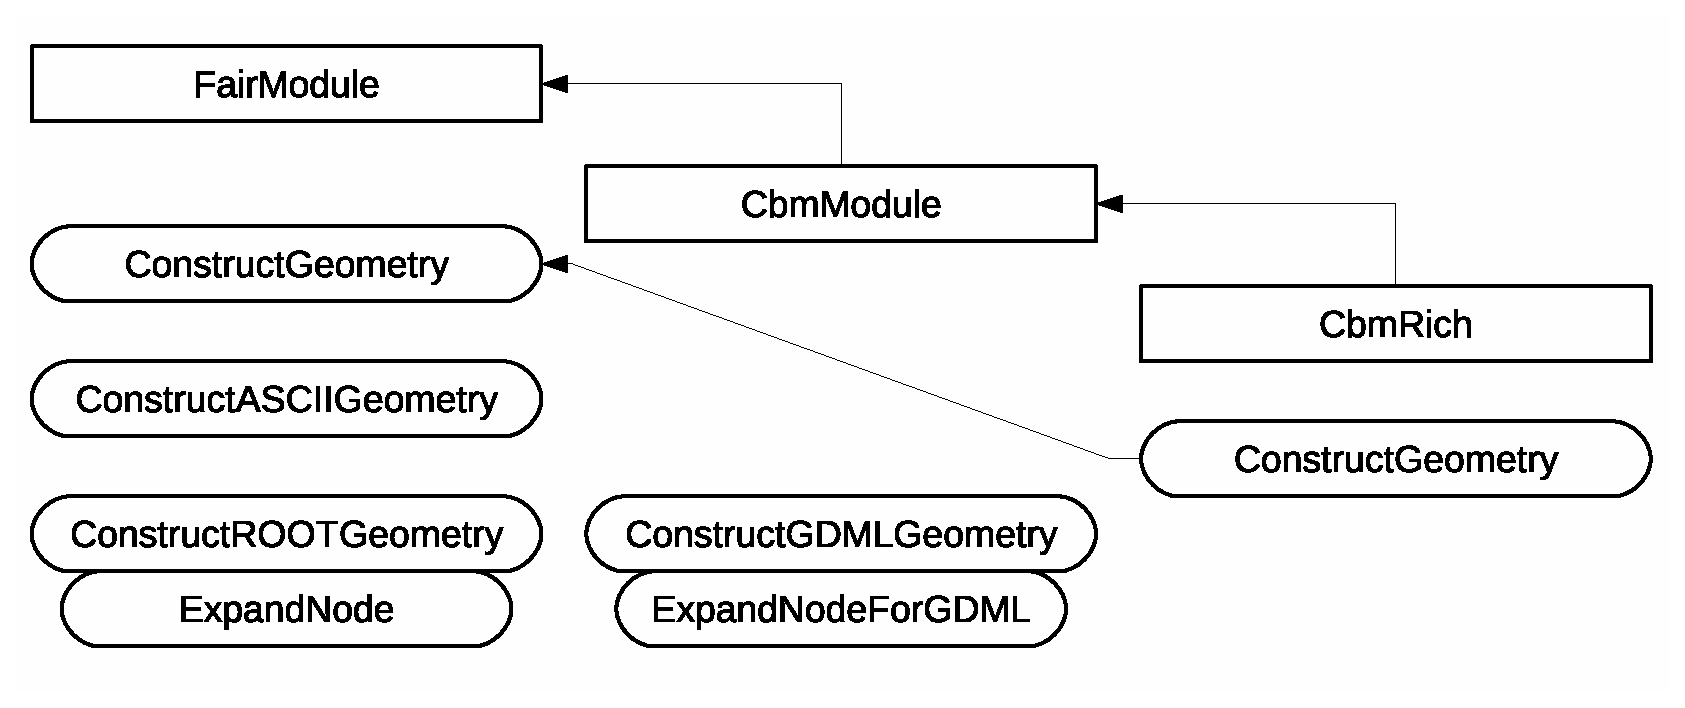
\includegraphics[width=0.7\textwidth]{pictures/FairModule_classes_after.eps}
\caption{Диаграмма классов CbmROOT после модификации.}
\label{fig:classesAfter}
\end{figure}

Введён промежуточный класс \classname{CbmModule}, имеющий 2 метода --- \methodname{ConstructGDMLGeometry} и вспомогательный \methodname{ExpandNodeForGDML}.

Добавлена ветвь условия, обеспечивающая вызов \classname{ConstructGDMLGeometry} в случае получения входного файла в формате GDML.

\begin{lstlisting}
void CbmRich::ConstructGeometry()
{
   TString fileName=GetGeometryFileName();
   if (fileName.EndsWith(".geo")) {
      ConstructGEOGeometry();
   } else if (fileName.EndsWith(".root")) {
      ConstructROOTGeometry();
   } else if (fileName.EndsWith(".gdml")) {
      ConstructGDMLGeometry(fposrot);
   } else {
      std::cout << "Geometry format not supported." << std::endl;
   }
}
\end{lstlisting}

Также для геометрии, импортированной из GDML, добавлена опциональная возможность позиционировать детектор непосредственно в макросе путём указания координат смещения и углов поворота. Данные параметры необязательны --- в случае их отсутствия детектор позиционируется по умолчанию. Для каждого элемента установки необходимо указать такие значения по умолчанию в заголовке класса. Данная процедура была выполнена для детектора RICH. Такая возможность позволяет продвинутому пользователю оперативно менять установку, а наличие значений по умолчанию ограждает неопытных пользователей от ошибок.

Все изменения были приняты и внесены в дистрибутив CbmROOT, также как и новая геометрия CBM RICH в форматах GDML и ROOT. Решено хранить как исходный GDML файл, так и ROOT файл, полученный в результате процедуры импорта GDML и экспорта в ROOT.

Таким образом, выполнена разработка модулей FairROOT для гибкой работы с форматом GDML, разработанные модули применены для обновления геометрии детектора RICH эксперимента CBM.

% Кусок о подсасывании описания материалов из внешнего файла
Стандартное применение GDML подразумевает, что в файле имеется полная информация о модели, в том числе и о материалах. Это означает, что при импорте GDML файла в GEANT4 или ROOT описание материалов будет взято из секции <materials>. На практике это оказывается очень неудобным, поэтому в экспериментальных пакетах, как например в CbmRoot, по умолчанию включена опция считывания из GDML только имена материала, игнорируя собственно описание. Однако в любом случае, для того чтобы GDML файл считался корректным с формальной точки зрения, для каждой ссылки должен существовать объект, на который эта ссылка указывает. В ``Builder'' мы используем минимальное dummy \todo описание, чтобы соблюсти правила XML файла, а фактически используется внешняя база материалов.